\documentclass{article} 

\usepackage[utf8]{inputenc} 

\usepackage[T1]{fontenc}
\usepackage{wrapfig}
\usepackage{graphicx}

\usepackage{subfig}

\title{Evaluación 2}

\author{Ricardo Ruiz Hernández}

\date{26 de Abril, 2018}
 

\begin{document}

\maketitle 
\section{Introducción}
En esta evaluación se abordó el llamado "Atractor de Lorenz", mismo que es un sistema de ecuaciones diferenciales, cuyas soluciones son caóticas. Dichas ecuaciones son las siguientes:

\begin{equation}
\frac{dx}{dt}=\sigma (y-x)
\end{equation}
\begin{equation}
\frac{dy}{dt}= x(\rho -z)-y
\end{equation}
\begin{equation}
\frac{dz}{dt}=xy -\beta z
\end{equation}

\section{Análisis}
\subsection{Ejemplo 1}
Visualización del modelo canónico en 3D: 

\begin{center}
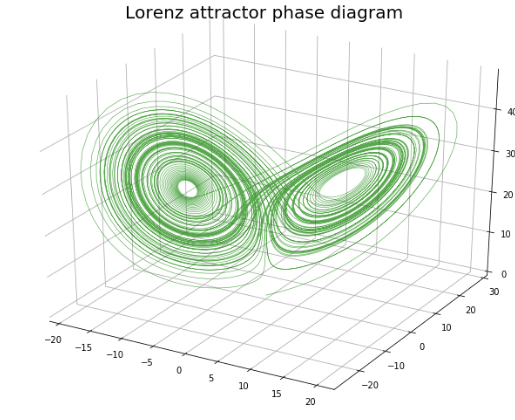
\includegraphics[scale=0.4]{Eval1.png}
\end{center}

Desde otras perspectivas:
\begin{center}
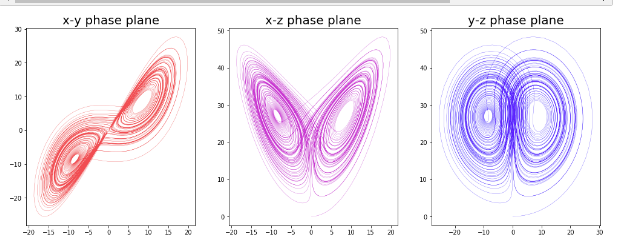
\includegraphics[scale=0.5]{Eval2.png}
\end{center}
En esta última se visualiza una gráfica con valores iniciales:
\begin{center}
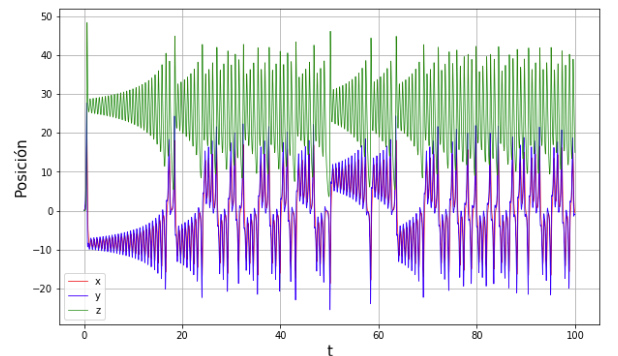
\includegraphics[scale=0.4]{Eval3.png}
\end{center}

\subsection{Ejemplo 2}
Esta gráfica de visualización es básicamente igual que la primera del ejemplo anterior, pero con diferencias en cuanto al tamaño:
\begin{center}
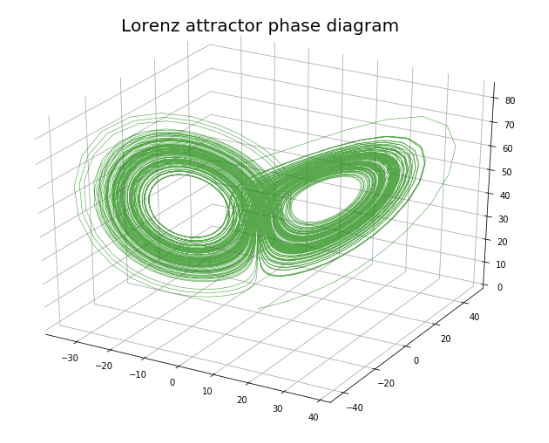
\includegraphics[scale=0.4]{Eval4.png}
\end{center}

\begin{center}
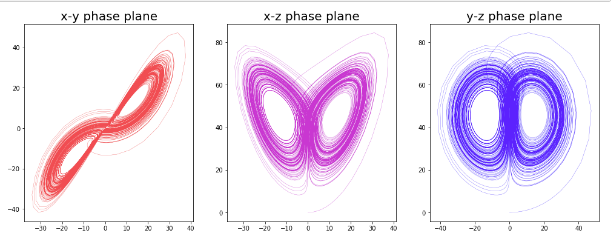
\includegraphics[scale=0.5]{Eval5.png}
\end{center}

\begin{center}
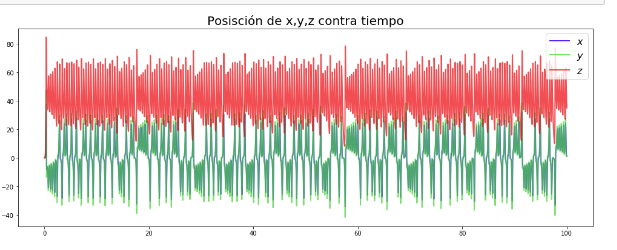
\includegraphics[scale=0.5]{Eval6.png}
\end{center}
\begin{center}
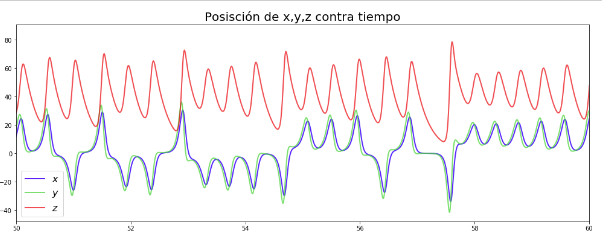
\includegraphics[scale=0.7]{Eval7.png}
\end{center}

\subsection{Ejemplo 3}
La última gráfica del atractor se encuentra orientada hacia los negativos del eje x, debido al cambio sufrido en rho.
\begin{center}
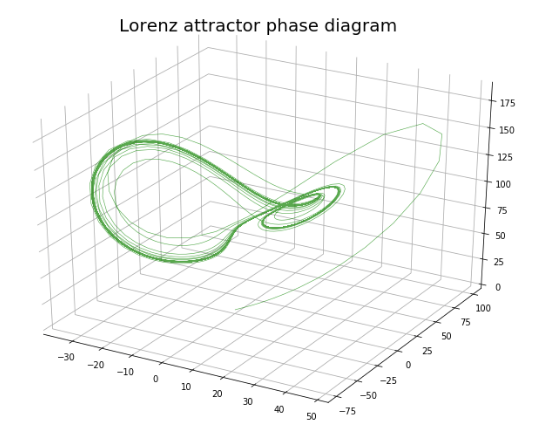
\includegraphics[scale=0.4]{Eval8.png}
\end{center}

En estas 3 gráficas se hace aún más evidente la no simetría:
\begin{center}
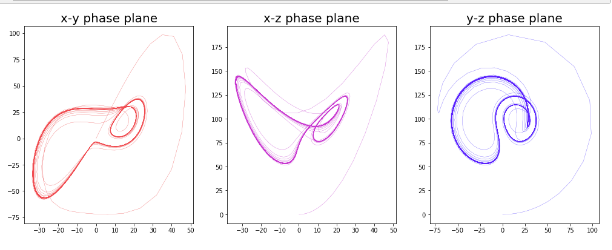
\includegraphics[scale=0.5]{Eval9.png}
\end{center}

\begin{center}
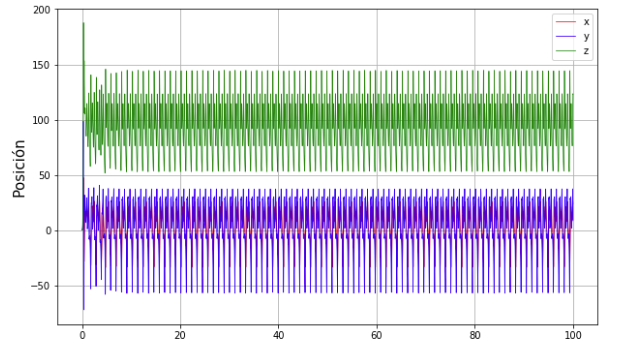
\includegraphics[scale=0.]{Eval10.png}
\end{center}

\section{Conclusión}
Siempre me ha parecido un tema de interés el caos, y está actividad me ilustró por medio de gráficas y analisis de ecuaciones lo que esto es. En términos generales, la evalución fue sencilla y contundente.

\section{Bibliografía}
\begin{itemize}
\item Código de Animación del Atractor de Lorenz (2016). Geoff Boeing.26 de Abril del 2018. Página:  https://github.com/gboeing/lorenz-system/blob/master/lorenz-system-attractor-animate.ipynb
\item Animating the Lorenz Attractor with Python (2016). Geoff Boeing. 26 de Abril del 2018. Página: http://geoffboeing.com/2016/12/animating-lorenz-attractor-python/
\item Código de Visualización del Atractor de Lorenz (2016). Geoff Boeing. 26 de Abril del 2018. Página:  https://github.com/gboeing/lorenz-system/blob/master/lorenz-system-attractor-visualize.ipynb

\end{itemize}



\end{document}